\chapter{Analýza}
V této kapitole bude probrána specifikace, požadavky na API a také požadavky na celkové fungování hry. Část je také věnována analýze již existujících herních API.

Cílem této práce je vytvořit zdokumentované jednotné API, které bude používáno jak uživatelským prostředím, tak i administrátorským rozhraním.

\section{Analýza již existujících herních API}

Tato část se věnuje představení již existujících online her s evolucí herních situací, která se ukládá mezi sezeními. Těchto her ovšem není mnoho -- většina webových online her nenutí uživatele k přihlášení a také nepodporuje postup či evoluce situací. Takovéto prémiové hry mívají většinou spíše formu desktopových aplikací a v takovém případě by se bohužel špatně analyzovala odcházející a přicházející komunikace.
Byla mi ovšem doporučena jedna hra, která je vytvořená přímo pro hraní za pomocí API, proto jsem se rozhodl tuto hru analyzovat a zjistit, jaké funkce a požadavky by mělo API pro tuto hru splňovat.

\subsection{SpaceTraders API}\label{sub:SpaceTraders}
SpaceTraders je hra založená na REST API, ve které hráči kontrolují a rozšiřují své flotily vesmírných lodí a za jejich pomocí objevují, obchodují a probíjí si vlastní cestu skrz galaxii. Hra je určena pro nadšence, kteří jsou vybízeni vytvořit si vlastní frontend a případně herní mechaniky automatizovat přes jakýkoli jazyk, což může sloužit i jako příjemný nástoj, jak se naučit práci s API nebo nový programovací jazyk. API je zdokumentováno za pomocí technologií OpenAPI a Stoplight. \cite[]{spacetraders}

Pro dotazování hra využívá jak parametrů dotazu tak proměnných v dotazované URL\@.

Token se vkládá do hlavičky ve formátu \texttt{'Authorization: Bearer INSERT\_TOKEN\_HERE'}. Tento token má formu zakódovaného JWT \sectionref{sec:jwt} objektu pomocí RS256.
Jeho dekódovaný text je zobrazen na obrázku \ref{fig:jwt_spacetraders}.

\begin{figure}[!ht]
    \centering
    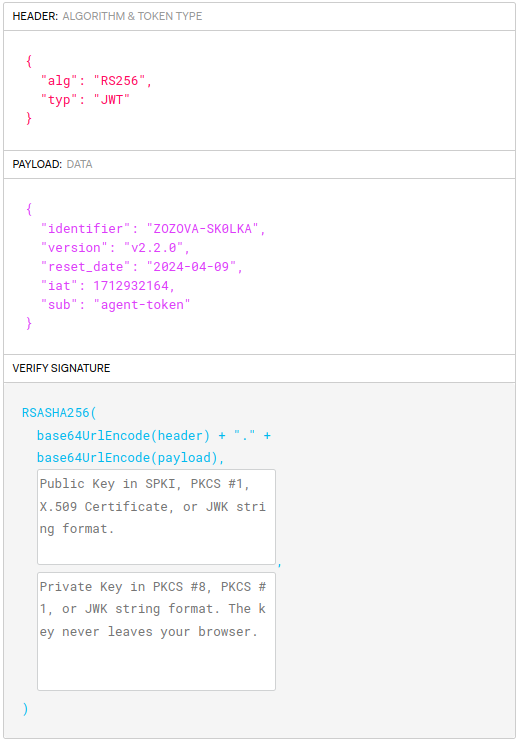
\includegraphics[width=0.5\textwidth]{figures/spaceTraders/jwt.png}
    \caption{Dekódovaný token ze hry SpaceTraders\cite[JWT decoder]{jwt_decoder}}
    \label{fig:jwt_spacetraders}
\end{figure}

Hra nejprve vyžaduje registraci přes endpoint \texttt{/v2/register}. Ten vrátí údaje o novém agentovi spolu s autentizačním tokenem \coderef{code:space_login}[řádek 3], se kterým se uživatel bude dále ověřovat ve všech následujících požadavcích.

\begin{listing}[!ht]
    \inputminted[breaklines]{json}{resources/code/spaceTraders/login.jsonc}
    \caption{Odpověď na požadavek na registraci\protect\footnotemark}
    \label{code:space_login}
\end{listing}
\footnotetext{Velká část dat musela být pro přehlednost smazána}

Jako odpověď se zde používá formát JSON, který obsahuje především objekt \texttt{data} a poté dodatečné objekty jako třeba \texttt{meta}, ve kterých mohou být další informace jako stránkování. % TODO odkaz na stránkování
Status je použit v souladu s klasickým výkladem statusových kódů % TODO odkaz na ty pravidla někde v restku
a dále je obsahu rozšířen o konkrétní popis chyby v daném požadavku. Příklad je vidět na výpisu \ref{code:space_error}, kde je zobrazena chyba při požadavku na odlet na jinou planetu, neboť loď není na orbitě.


\begin{listing}[ht!]
    \inputminted[breaklines]{json}{resources/code/spaceTraders/error_response.jsonc}
    \caption{Výpis chyby při požadavku odletět na jinou planetu}
    \label{code:space_error}
\end{listing}

\section{Specifikace požadavků}
Pomocí výše provedené analýzy API existujících her, vyčlenění požadavků na funkcionality hry ze strany ostatních členů týmu a za pomocí analýzy dostupných nástrojů pro tvorbu API byly vytyčeny požadavky a funkce, které by mělo API modelové hry podporovat. Jedná se především o CRUD operace se základními objekty, jejich filtrování, stránkování a lazy load. API by taktéž mělo podporovat přihlašování a obranu před základními typy útoků jako je SQL injection, DDOS a DOS útok nebo neoprávněný přístup díky chybám v API.

API by taktéž mělo podporovat validaci všech vstupních dat (rozsahy vstupních hodnot, filtrace speciálních znaků, kontrola správného postupu operací při hraní hry) a mělo by mít odpovídající koncové body pro samotné hraní hry.

\subsection{Funkční požadavky}
Nyní si představíme funkční požadavky na API, které předložili ostatní členové týmu. Tyto požadavky se měnily a rozšiřovaly spolu s průběhem návrhu i implementace. Některé požadavky, které vzešly primárně z backoffice se využívají ve frontendu a případně i naopak.

\subsubsection*{Požadavky, které byly vyčleněny primárně ze strany backoffice}

\begin{enumerate}[label=\textbf{F\arabic*}:, leftmargin=*, align=left]
    \item \textbf{CRUD operace} -- Nad základními objekty, se kterými se bude často pracovat, a upravovat pomocí endpointů. Těmito objekty jsou \texttt{akce, efekty, předměty, charaktery a jejich vlastnosti, dobrodružství, kampaň, obchody, nepřátelé, překážky, lokace} a \texttt{části lokace}
    \item \textbf{Filtrování} -- Možnost vyhledat objekty podle vstupních parametrů u koncových bodů, které poskytují seznam objektů.
    \item \textbf{Lazy load} -- Způsob načítání dat, který umožňuje vracet pouze daný objekt bez jeho závislostí, případně vrácení pouze těch závislostí, které se určí. Výsledkem je rychlejší zpracování a menší objem přesunutých dat, když uživatel tyto závislosti nepotřebuje. Namísto objektu se tedy vrátí jen jeho identifikátor.
    \item \textbf{Stránkování} -- Další způsob předávání dat, který umožní jejich postupné zpracování, což vede ke zkrácení času potřebného k vyhodnocení požadavku jak v API tak ve zobrazovací části.
    \item \textbf{Caching} -- Již jednou zpracovaná data z databáze není třeba znovu získávat z databáze, pokud nedošlo ke změně. Tato funkcionalita umožní násobně rychlejší odezvu pro opakované získávání stejných dat.
    \item \textbf{Administrátorská práva} -- Ne všichni mohou mít přístup pro úpravu dat v databázi. Díky administrátorským přihlašovacím údajům a následnému tokenu se budou moci upravovat a vkládat data do databáze pouze s odpovídajícím ověřením.
    \item \textbf{Validace} -- Data vkládaná do databáze budou validována a případně vrátí chybovou hlášku, podle které bude možno snadno identifikovat chybu vstupních dat a následně ji opravit.
\end{enumerate}


\subsubsection*{Požadavky primárně ze strany uživatelského prostředí}

\begin{enumerate}[label=\textbf{F\arabic*}:, leftmargin=*, align=left]
    \item \textbf{Získávání objektů} -- Bude umožněno získávat jakékoliv objekty, které neobsahují herní data či jiné citlivé informace, přímo z databáze.
    \item \textbf{Podpora herního průběhu} -- Uživatel bude moci projít celým soubojem a interagovat s entitami v něm za pomocí řady validovaných a přehledně uspořádaných koncových bodů.
    \item \textbf{Zamezení zneužití} -- Postup operací v herním průběhu bude kontrolován tak, aby se zamezilo případnému zneužití nebo obcházení pravidel hry.
    \item \textbf{Přihlášení} -- Uživatel se bude moci přihlásit a získat token pro ověření v dalších požadavcích.
    \item \textbf{Herní data} -- Uživatel bude mít pod svým účtem uložený postup hry a bude moci pokračovat tam, kde skončil. Dále bude mít možnost vytvářet nové postavy pro kampaně a také nová dobrodružství.
    \item \textbf{Validace} -- Obsah vstupních dat bude validován a případně vrátí smysluplnou chybovou hlášku.
    \item \textbf{Obrázky} -- Bude možné získat obrázek z url adresy přiložené k objektu, případně v požadavku specifikovat jeho velikost.
\end{enumerate}



\subsection{Nefunkční požadavky}
Dále je důležité vyhradit si nefunkční požadavky. Jejich vznik je stejný jako požadavky funkční, byly sestrojovány postupně s vývojem na základě zkušeností a požadavků ostatních členů týmu.


\begin{enumerate}[label=\textbf{F\arabic*}:, leftmargin=*, align=left]
    \item \textbf{Rozdělení API na dvě části} -- Z důvodu spolupráce na API s jinými členy týmu, především herním systémem, který pro svůj chod využívá stejných modelů, bylo rozhodnuto, že herní logika i mapování bude v jednom projektu. Tomu tedy musí být přizpůsobena i spolupráce a podpůrné technologie.
    \item \textbf{Dokumentace} API bude zdokumentováno za pomocí OpenAPI a pro vizuální zobrazení koncových bodů bude použit Swagger, který zároveň poslouží jako skvělé ladící rozhraní.
    \item \textbf{Hosting} API bude stejně jako ostatní části projektu hostováno na veřejných serverech.
    \item \textbf{Přehlednost} Koncové body API by měly být samopopisující a snadno pochopitelné.
    \item \textbf{Standardizovanost} API se bude držet ověřených dobrých praktik z praxe a bude udržovat jednotnost a standardizovanost.
\end{enumerate}

